\section{Obvody buzené časově proměnnými zdroji}

\subsection{Sériový RL obvod buzený harmonický zdrojem}

\begin{figure}[h!]
\centering
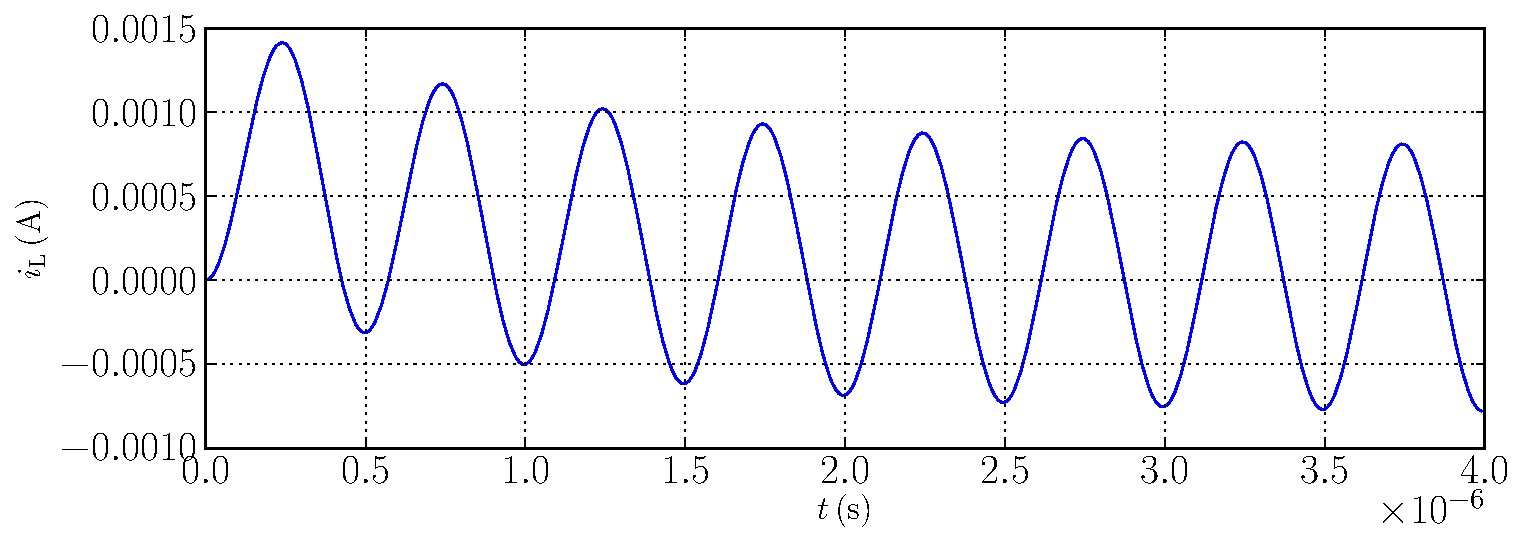
\includegraphics[width=13cm]{prechodne_jevy/specialni/obvod_rl_harmonicky_proud.pdf}
\caption{Sériový RL obvod: proud induktorem}
\label{fig:obvod_rl_proud}
\end{figure}

\subsection{RC obvod buzený obdélníkovým signálem}

$$
\frac{u_0 - u_\mathrm{C}}{R_1} - C \frac{\dif u_\mathrm{C}}{\dif t} - u_\mathrm{C} = 0
$$

\begin{figure}[h!]
\centering
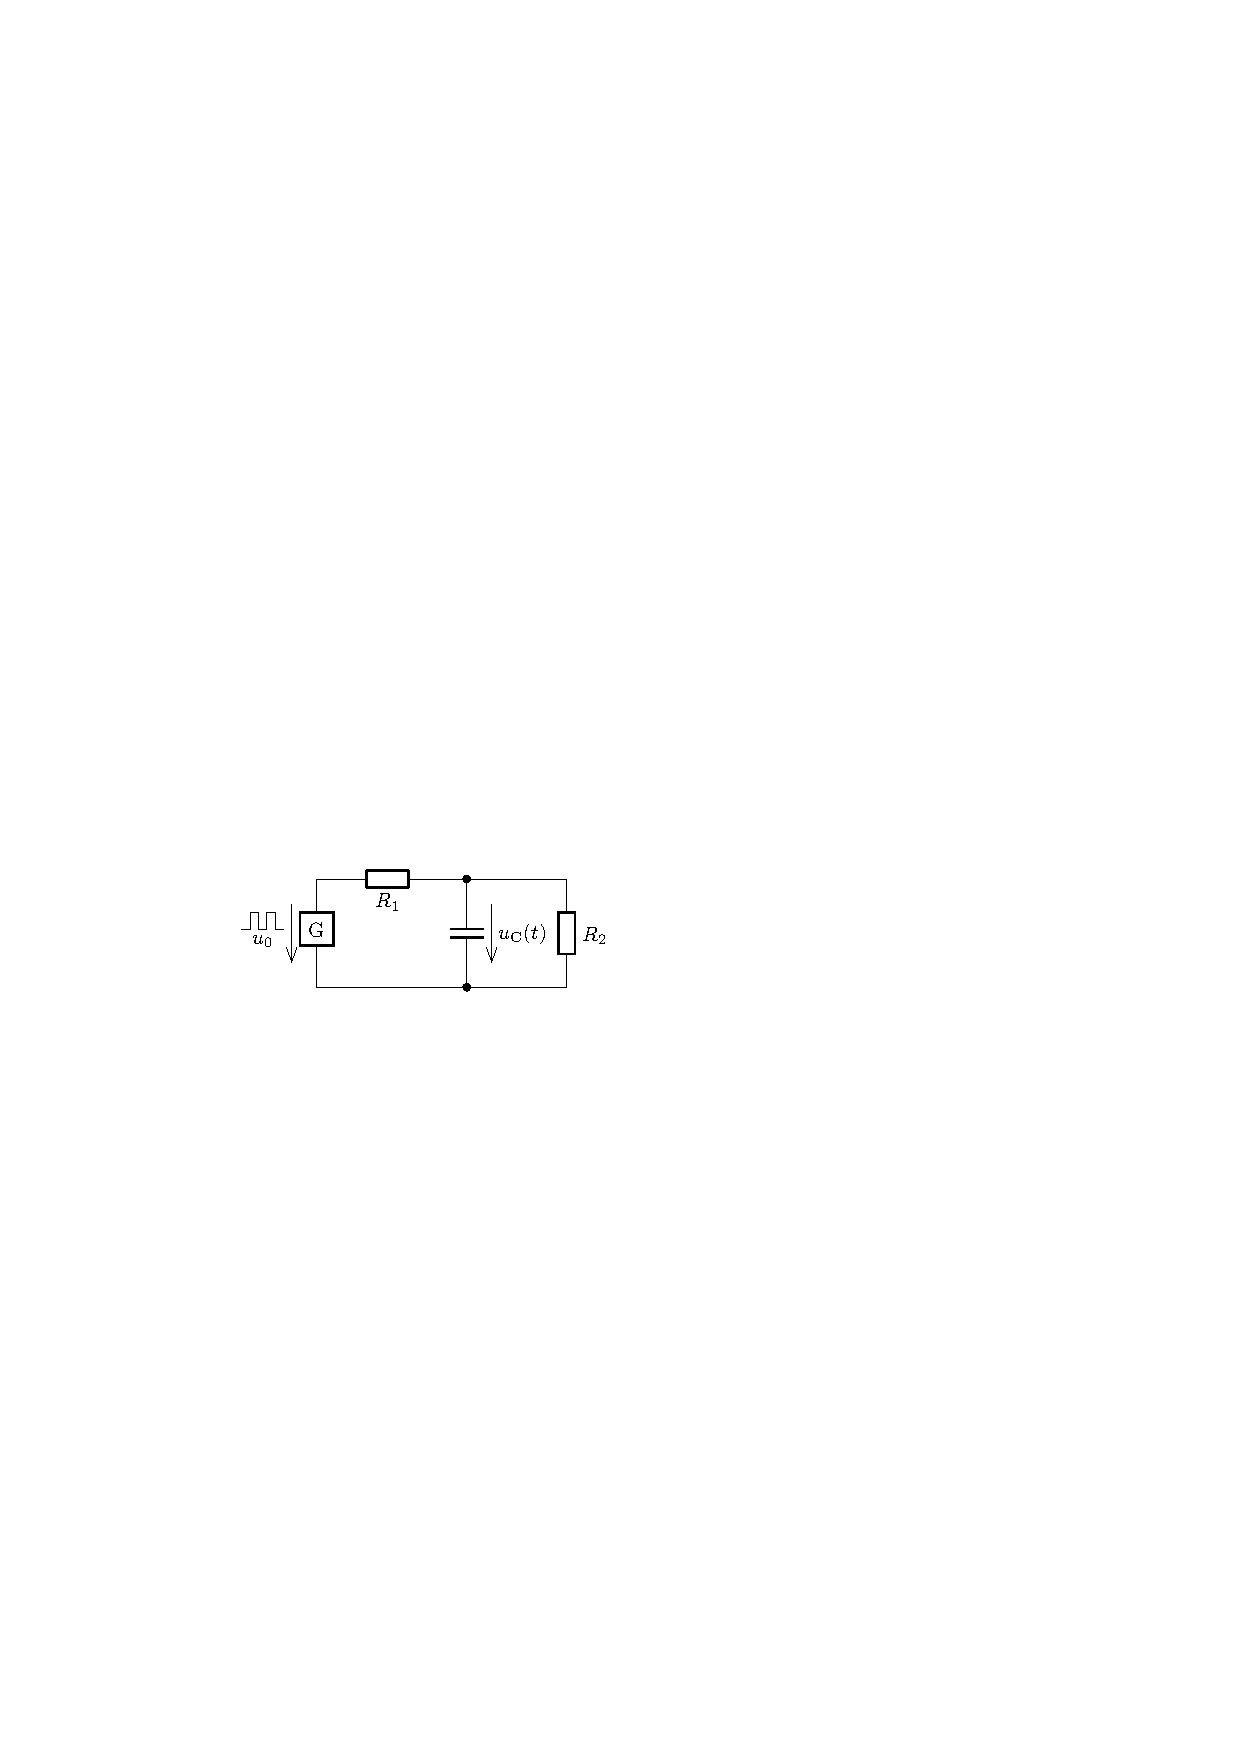
\includegraphics[]{prechodne_jevy/specialni/rc_obdelnik.pdf}
\caption{Sériový RL obvod: proud induktorem}
\label{fig:rc_proud}
\end{figure}

\begin{figure}[h!]
\centering
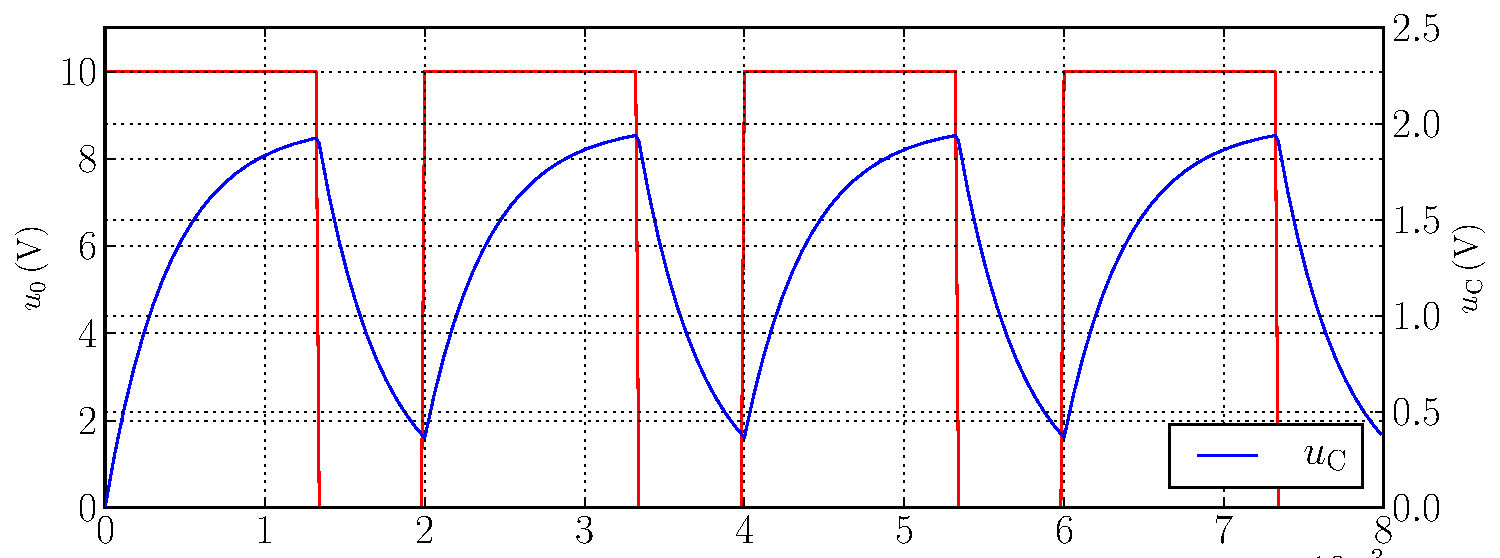
\includegraphics[width=13cm]{prechodne_jevy/specialni/obvod_rc_obdelnik.pdf}
\caption{Obvod prvního řádu buzený obdélníkovým signálem (modrá barva -- napětí $u_\mathrm{C}$, červená barva -- napětí $u_\mathrm{0}$}
\label{fig:obvod_rc_napeti}
\end{figure}
